Introducidos en 1959 independientemente por Rene de la Briandais y Edward Fredkin un\emph{Trie} es una estructura de datos de tipo árbol que permite la recuperación 
de información (de ahí su nombre del inglés \emph{reTRIEval}). La información almacenada en un \emph{Trie} es un conjunto de claves, donde una clave es una secuencia 
de símbolos pertenecientes a un alfabeto. Las claves son almacenadas en las hojas del árbol y los nodos internos son pasarelas para guiar la búsqueda. El árbol se 
estructura de forma que cada letra de la clave se sitúa en un nodo de forma que los hijos de un nodo representan las distintas posibilidades de símbolos diferentes 
que pueden continuar al símbolo representado por el nodo padre. Por tanto la búsqueda en un \emph{Trie} se hace de forma similar a como se hacen las búsquedas en un 
diccionario: 

\emph{Se empieza en la raíz del árbol. Si el símbolo que estamos buscando es A entonces la búsqueda continúa en el subárbol asociado al símbolo A que cuelga de la raíz. Se sigue de forma análoga hasta llegar al nodo hoja. Entonces se compara la cadena asociada al nodo hoja y si coincide con la cadena de búsqueda entonces la búsqueda ha terminado en éxito, si no entonces el elemento no se encuentra en el árbol.}

La estructura de datos \emph{Trie} se define como una estructura de datos basada en árboles que se utiliza para almacenar una colección de cadenas y realizar operaciones de búsqueda eficientes en ellas. 

\emph{Trie} sigue una propiedad de que si dos cadenas tienen un prefijo común, entonces tendrán el mismo ancestro en el \emph{Trie}.

Ahora ya sabemos que \emph{Trie} tiene una estructura en forma de árbol. Por eso, es muy importante conocer sus propiedades. A continuación se muestran algunas propiedades importantes de la estructura de datos \emph{Trie}:

\begin{itemize}
	\item Hay un nodo raíz en cada \emph{Trie}.
	\item  Cada nodo de un \emph{Trie} representa una cadena y cada arista representa un carácter.
	\item  Cada nodo consta de \emph{hashmaps} o una matriz de punteros, y cada índice representa un carácter y una bandera para indicar si alguna cadena termina en el nodo actual.
	\item La estructura de datos \emph{Trie} puede contener cualquier número de caracteres, incluidos alfabetos, números y caracteres especiales. Por ejemplo para cadenas con caracteres a-z  solo se necesitan 26 punteros para cada nodo, donde el índice 0 representa los caracteres \emph{a} y el índice 25 representa los caracteres \emph{z}.
	\item  Cada ruta desde la raíz hasta cualquier nodo representa una palabra o cadena.
\end{itemize}

\subsection{Representación de \emph{Trie}}

Hay varias formas de representar un Trie, que corresponden a diferentes compensaciones entre el uso de la memoria y la velocidad de las operaciones. La forma básica es la de un conjunto vinculado de nodos, donde cada nodo contiene una array de punteros secundarios, uno para cada símbolo en el alfabeto (por lo que para el alfabeto inglés, uno almacenaría 26 punteros secundarios y para el alfabeto de bytes, 256 punteros). El nodo \emph{Trie} también mantiene un indicador que especifica si corresponde o no al final de la clave.

Como se ilustra en la siguiente figura, cada clave se representa en el \emph{Trie} como un camino desde la raíz hasta el nodo interno o una hoja:

% TODO: \usepackage{graphicx} required
\begin{figure}[h!]
	\centering
	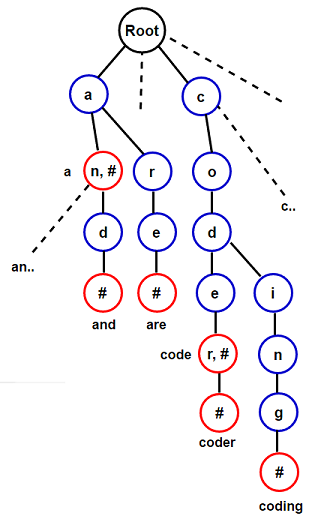
\includegraphics[width=0.4\linewidth]{img/Trie}
	\label{fig:trie}
\end{figure}

Veamos cómo se almacena una palabra \emph{and} y \emph{are} en la estructura de datos de \emph{Trie}:

\begin{enumerate}
	\item Almacene \emph{and} en la estructura de datos \emph{Trie}:
	\begin{itemize}
		\item La palabra \emph{and} comienza con \emph{a}, por lo que inicilizaremos el nodo hijo que representa \emph{a} con memoria en el nodo \emph{Trie}, que representa el uso de \emph{a}.
		\item Después de colocar el primer carácter, para el segundo carácter nuevamente hay 26 posibilidades, así que desde el nodo \emph{a}, nuevamente hay un nuevo nodo \emph{n}, para almacenar y representar el segundo carácter.
		\item El segundo carácter es \emph{n}, así que de \emph{a}, nos moveremos a \emph{n}.
		\item Después de \emph{n}, el tercer carácter es \emph{d},nuevamente hay un nuevo nodo \emph{d} que tiene como padre el nodo \emph{n}, para almacenar y representar el tercer carácter. Para dicho nodo se establece una marca que indica que desde la raíz del \emph{Trie} hasta ese nodo hay una cadena.
	\end{itemize}
	\item Almacene \emph{are} en la estructura de datos \emph{Trie}:
	\begin{itemize}
		\item La palabra \emph{are} comienza con \emph{a} y el nodo \emph{a} en el nodo raíz ya se ha creado. Entonces, no es necesario volver a crarlo, solo muévase al nodo \emph{a} en Trie.
		\item Después de colocar el primer carácter, para el segundo carácter nuevamente hay 26 posibilidades de las cuales ya existe uno previamente \emph{n}, así que desde el nodo \emph{a}, nuevamente hay un nuevo nodo \emph{r}, para almacenar y representar el segundo carácter.
		\item El segundo carácter es \emph{r}, así que de \emph{a}, nos moveremos a \emph{r}.
		\item Después de \emph{r}, el tercer carácter es \emph{e},nuevamente hay un nuevo nodo \emph{e} que tiene como padre el nodo \emph{r}, para almacenar y representar el tercer carácter. Para dicho nodo se establece una marca que indica que desde la raíz del \emph{Trie} hasta ese nodo hay una cadena.
	\end{itemize}
\end{enumerate}

\subsection{Operaciones}

El \emph{Trie} puede presentar varias operaciones en dependencia de la situación donde vaya ser aplicado, pero al menos las operaciones de \emph{Inserción}, \emph{Búsqueda} y \emph{Eliminación} son las más utilizadas o sirven de base de implementación para otras operaciones que puede ser soportada por la estructura. 

\subsubsection{Inserción}

Se procede recorriendo el \emph{Trie} de acuerdo con la string que se va a insertar, y luego agrega nuevos nodos para el sufijo de la string que no está contenido en el \emph{Trie}. Esta operación se utiliza para insertar nuevas cadenas en la estructura de datos de Trie. Veamos cómo funciona esto:

Intentemos insertar \emph{and} y \emph{ant} en este Trie:  

% TODO: \usepackage{graphicx} required
\begin{figure}[h!]
	\centering
	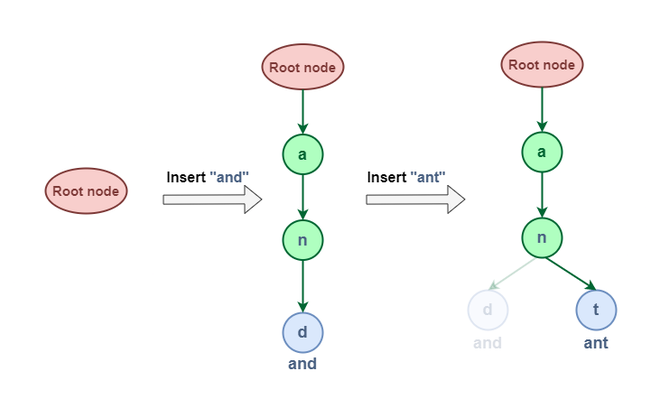
\includegraphics[width=0.7\linewidth]{img/trie_insert}
	\label{fig:trieinsert}
\end{figure}

De la representación de inserción anterior, podemos ver que la palabra \emph{and} y \emph{ant} han compartido algún nodo común (es decir, \emph{an}), esto se debe a la propiedad de la estructura de datos \emph{Trie} de que si dos cadenas tienen un prefijo común entonces tendrán el mismo ancestro en el \emph{Trie}.

Ahora intentemos insertar \emph{dad} y \emph{do}:

\begin{figure}[h!]
	\centering
	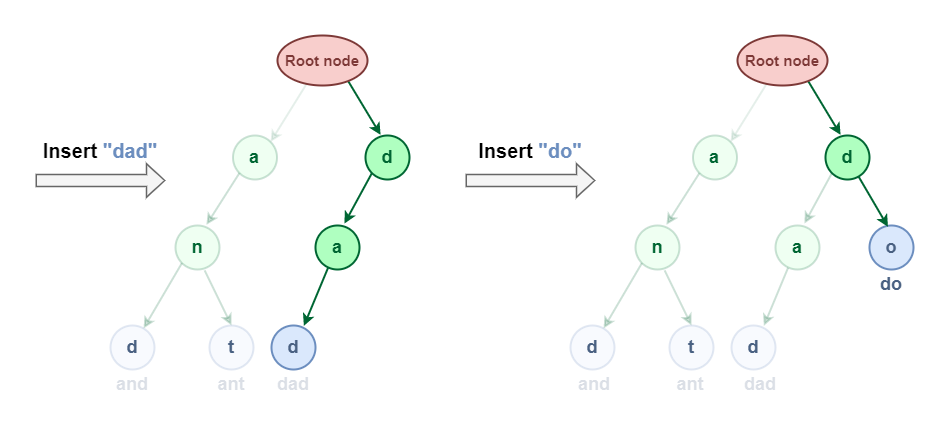
\includegraphics[width=0.7\linewidth]{img/trie_insert_a}
	\label{fig:trieinserta}
\end{figure}

Algoritmo de inserción en la estructura de datos \emph{Trie}:

\begin{enumerate}
	\item Definir una función insert(TrieNode root, string word) que tomará dos parámetros uno para la raíz y otro para la cadena que queremos insertar en la estructura de datos \emph{Trie}.
	\item Ahora tome otro puntero \emph{currentNode} e inicialícelo con el nodo raíz.
	\item Itere sobre la longitud de la cadena dada y verifique si el valor es NULL o no en el arreglo de punteros en el carácter actual de la cadena.
	\begin{itemize}
		\item Si es NULL entonces, crea un nuevo nodo y apunta el carácter actual a este nodo recién creado.
		\item  Mueva el \emph{currentNode} al nodo recién creado.
	\end{itemize}
	\item Finalmente, incremente el número de palabras del último nodo actual, esto implica que hay una cadena que termina en nodo actual.
	
\end{enumerate}

\subsubsection{Búsqueda}

La operación de búsqueda en \emph{Trie} se realiza de manera similar a la operación de inserción, pero la única diferencia es que cada vez que encontramos que el arreglo de punteros en el nodo actual no apunta al carácter actual de la palabra, devuelve falso en lugar de crear un nuevo nodo. por ese carácter actual de la palabra.

Esta operación se utiliza para buscar si una cadena está presente en la estructura de datos Trie o no. Hay dos enfoques de búsqueda en la estructura de datos de \emph{Trie}.

\begin{enumerate}
	\item Encuentra si existe alguna palabra que comience con el prefijo dado en \emph{Trie}
	\item Encuentra si la palabra dada existe en \emph{Trie}. Es similar a la búsqueda de prefijos, pero además, debemos verificar si la palabra termina en el último carácter de la palabra o no.
\end{enumerate}

Hay un patrón de búsqueda similar en ambos enfoques. El primer paso para buscar una palabra dada en Trie es convertir la palabra en caracteres y luego comparar cada carácter con el nodo trie del nodo raíz. Si el carácter actual está presente en el nodo, avance a sus hijos. Repita este proceso hasta encontrar todos los caracteres.

\subsection{Eliminación}

Es un poco complicado La idea es eliminar la clave de forma ascendente utilizando recursión. Se debe tener especial cuidado al eliminar la clave, ya que puede ser el prefijo de otra clave, o su prefijo puede ser otra clave en \emph{Trie}. Hay tres casos cuando se elimina una palabra de \emph{Trie}.

\begin{enumerate}
	\item \textbf{La palabra eliminada es un prefijo de otras palabras en \emph{Trie}:} Como se muestra en la siguiente figura, la palabra eliminada \emph{an} comparte un prefijo completo con otra palabra \emph{and} y \emph{and}. Una solución fácil para realizar una operación de eliminación en este caso es simplemente disminuir el recuento de palabras en 1 en el nodo final de la palabra.
	
	% TODO: \usepackage{graphicx} required
	\begin{figure}[h!]
		\centering
		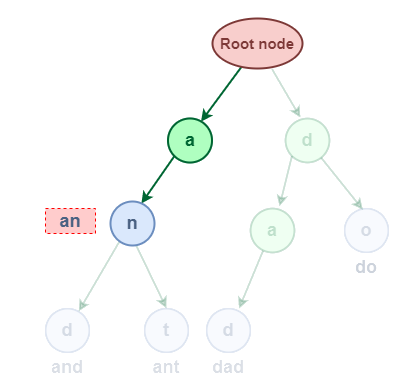
\includegraphics[width=0.35\linewidth]{img/case1_delete}
		\caption{La palabra eliminada es un prefijo de otras palabras en \emph{Trie}}
		\label{fig:case1delete}
	\end{figure}
	
	\item \textbf{La palabra eliminada comparte un prefijo común con otras palabras en \emph{Trie}:} Como se muestra en la siguiente figura, la palabra eliminada \emph{and} tiene algunos prefijos comunes con otras palabras \emph{ant}. Comparten el prefijo \emph{an}. La solución para este caso es eliminar todos los nodos desde el final del prefijo hasta el último carácter de la palabra dada.
	
		\begin{figure}[h!]
		\centering
		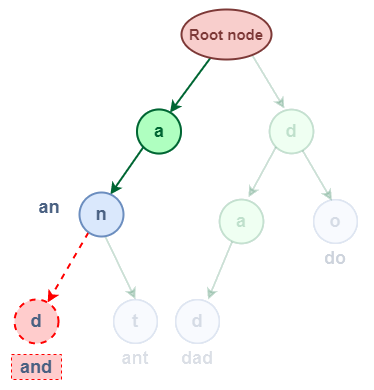
\includegraphics[width=0.35\linewidth]{img/case2_delete}
		\caption{La palabra eliminada comparte un prefijo común con otras palabras en \emph{Trie}}
		\label{fig:case1delete2}
	\end{figure}
	
	\item \textbf{La palabra eliminada no comparte ningún prefijo común con otras palabras en \emph{Trie}:} Como se muestra en la siguiente figura, la palabra \emph{geek} no comparte ningún prefijo común con ninguna otra palabra. La solución para este caso es simplemente eliminar todos los nodos.
	
			\begin{figure}[h!]
			\centering
			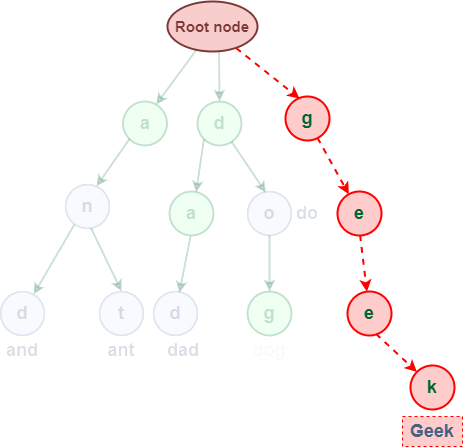
\includegraphics[width=0.35\linewidth]{img/case3_delete}
			\caption{La palabra eliminada no comparte ningún prefijo común con otras palabras en \emph{Trie}}
			\label{fig:case1delete3}
		\end{figure}
\end{enumerate}


Los \emph{Trie} puede ser visto con un árbol de búsqueda y presenta un grupo de ventajas sobre los árboles de búsqueda binaria  como son:

\begin{itemize}
	\item Búsqueda de claves más rápida. La búsqueda de una clave de longitud $M$ tendrá en el peor de los casos un coste de O($M$). Un árbol de búsqueda binaria tiene un coste de O ($M\log N$), siendo $N$ el número de elementos del árbol, ya que la búsqueda depende de la profundidad del árbol, logarítmica con el número de claves.
	\item Menos espacio requerido para almacenar gran cantidad de cadenas pequeñas, puesto que las claves no se almacenan explícitamente.
	\item Mejor funcionamiento para el algoritmo de búsqueda del prefijo más largo
\end{itemize} 